\section{Grounding Natural Language Instructions}
\label{sec:background}
Grounding natural language addresses the problem of understanding the meaning of a command within the current world configuration containing numerous objects. For example, grounding the command ``move to the cube" is inferring 1) the cube object in the world configuration, 2) the feasible region near the cube, and 3) the act of going towards the feasible region. Accordingly, let $\boldsymbol{\lambda}$ be the natural language command, let $\Gamma$ be the set of groundings that correspond to semantic notions such as objects, locations, regions, paths, or actions the robot can take, and let $\Upsilon$ denote the physical workspace of the robot that aggregates metric and semantic information about the constituent objects. Then, the symbol grounding problem can be formulated as %finding the correct association between the phrases   in the command and the obje 
\begin{equation}
\boldsymbol{\gamma}^* = \argmax_{\boldsymbol{\gamma} \in \Gamma^{|\boldsymbol{\lambda}|}} p(\boldsymbol{\gamma}|\boldsymbol{\lambda},\Upsilon),
\label{eq:max_ground_prob}
\end{equation}
where $\boldsymbol{\lambda}$ is a vector of phrases from the set $\Lambda$ and ${\Lambda = \{\text{English phrases}\}}$ denotes what phrases natural language sentences may be composed of; $|\boldsymbol{\lambda}|$ is the length of the command; $\boldsymbol{\gamma} \in \Gamma^{|\boldsymbol{\lambda}|}$ is a vector of groundings with a length of $|\boldsymbol{\lambda}|$; and the optimal vector of groundings $\boldsymbol{\gamma}^*$ is the one with maximum likelihood, given a command $\boldsymbol{\lambda}$ and a world model $\Upsilon$.

One efficient way of solving Eqn.~\eqref{eq:max_ground_prob} can be achieved via the Distributed Correspondence Graph (DCG) \cite{dcg}. This model is structured according to the hierarchical structure of the language command. For example, the parse structure of the instruction ``move to the cube" is illustrated in Fig.~\ref{fig:parse_tree}. Accordingly, the goal becomes to find the correct associations between ``move", ``to", ``the cube" and objects, regions in the world. 
%To this end, 
%% Before proceeding further, one must define the domains over which the grounding problem may be solved.
%the symbol grounding problem can be formulated as
%\begin{equation}
%\boldsymbol{\gamma}^* = \argmax_{\boldsymbol{\gamma} \in \Gamma^{|\boldsymbol{\lambda}|}} p(\boldsymbol{\gamma}|\boldsymbol{\lambda},\Upsilon),
%\label{eq:max_ground_prob}
%\end{equation}


%the cartesian product of the set of objects (i.e., $\boldsymbol{\Gamma^O} \subset \boldsymbol\Gamma$) and the object attributes (e.g., color, location), which represents the world model in which the phrases may be grounded. 

%In the general formulation of the grounding problem, three sets must be considered: ${\Gamma = \{\text{symbolic actions and objects\}}}$ is the set of groundings, which represents what phrases may be grounded to; ${\Lambda = \{\text{English phrases}\}}$ is the set of phrases, which represents what phrases natural language sentences may be composed of; and ${\Upsilon = \Gamma^O \times \{\text{object attributes}\} }$ is the cartesian product of the set of objects (i.e., $\Gamma^O \subset \Gamma$) and the object attributes (e.g., color, location), which represents the world model in which the phrases may be grounded. 

%Given a natural language command $\boldsymbol{\lambda}$, which is a vector of phrases from the set $\Lambda$ and has a length of $|\boldsymbol{\lambda}|$, 
%%\indent Using these domains, it is possible to formulate 
%the general grounding problem can be formulated as a probability maximization problem%, shown in Equation~\ref{eq:max_ground_prob},
%\begin{equation}
%\boldsymbol{\gamma}^* = \argmax_{\boldsymbol{\gamma} \in \Gamma^{|\boldsymbol{\lambda}|}} p(\boldsymbol{\gamma}|\boldsymbol{\lambda},\Upsilon),
%\label{eq:max_ground_prob}
%\end{equation}
%where $\boldsymbol{\gamma} \in \Gamma^{|\boldsymbol{\lambda}|}$ is a vector of groundings with a length of $|\boldsymbol{\lambda}|$, and $\Upsilon$ denotes the world model. 
%$\gamma \in \Gamma$, $\boldsymbol{\lambda}$ as a vector of phrases $\lambda \in \Lambda$ and world model $\Upsilon$. 

In the DCG model, the domains of $\Gamma$ and $\Lambda$ are defined a priori, and $\Upsilon$ represents the world model that contains the locations and identities of objects perceived by the robot. %in \eqref{eq:max_ground_prob} include the elements from previously seen examples. % While the general formulation allows any possible grounding, phrase, or world model, the domains of $\Gamma$, $\Lambda$, and $\Upsilon$ are shrunk in existing solutions to the grounding problem.
The set of phrases $\Lambda$ is assumed to only contain words that have appeared in the training examples. Similarly, the set of grounding symbols $\Gamma$ is assumed to contain 1) symbolic objects that the robot has been trained with, and 2) regions and motion constraints that are obtained by discretizing the perceived continuous space.  Additionally, the DCG model introduces another set of variables $\Phi$, and $\phi_{ij} \in \Phi$ is called a correspondence variable that refers to a binary relationship between the $i^{th}$ phrase $\lambda_i$ and the $j^{th}$ grounding variable $\gamma_{ij}$. The main assumption of the DCG model is that the grounding variables are conditionally independent from each other given the phrases. Overall, the DCG solves an inference problem as a search over the unknown correspondence variables as follows:  
%Moreover, solving \eqref{eq:max_ground_prob} is a hard combinatorial optimization problem due to the diversity in language and world.
% even though limited sets ($\Gamma$, $\Lambda$, and $\Upsilon$) are considered. 
%For example, the Generalized Grounding Graph (G3) model \cite{g3} is a factor graph that is trained from a corpus of labeled examples to ground language commands with objects, locations, and paths.  
%One way to tackle the complexity of solving \eqref{eq:max_ground_prob} is modeling it as an inference over a probabilistic graphical model based on the linguistic structure of the commands. In literature, there exists an efficient model called the Distributed Correspondence Graph (DCG) \cite{dcg}, which discretizes the continuous space of groundings ($\Gamma$) as regions and motion constraints and introduces binary correspondence variables ($\phi_{ij}$) relating the $i^{th}$ phrase $\lambda_i$ with the $j^{th}$ grounding variable $\gamma_{ij}$. The DCG model assumes the grounding variables as conditionally independent and solves an inference problem as a search over the unknown correspondence variables as follows: 
\begin{equation}
\label{eq:dcg_factored1}
\begin{split}
\boldsymbol{\phi}^* = \argmax_{\phi_{ij} \in \boldsymbol{\phi}} \prod_{i}^{| \boldsymbol{\lambda}|} \prod_{j}^{|\Gamma^i|} p(\phi_{ij}|\gamma_{ij},\lambda_i, \Phi_{c_{i}}, \Upsilon_{KP}),
\end{split}
\end{equation}
where $\lambda_i \in \Lambda_{KN}$ and $\Lambda_{KN}$ is the set of phrases with known (previously seen) words; $\Gamma^i$ is the set of grounding variables of $\lambda_i$ \footnote{If $\lambda_i$ is a noun phrase, the corresponding grounding set $\Gamma^i$ contains the objects in the world (i.e., $\Gamma^O$). If $\lambda_i$ is a verb phrase referring to the actions that the robot can take (e.g., ``move", ``pick"), then $\Gamma^i$ contains the regions discretized with respect to the objects under consideration (i.e., $\Gamma^{RO}$).}, $\phi_{ij}$ is the $j^{th}$ correspondence variable of $\lambda_i$; $\gamma_{ij}$ is the $j^{th}$ grounding of $\lambda_i$; $\Upsilon_{KP}$ denotes the world model consisting of the set of known perceived symbolic objects and regions; and  $\Phi_{c_{i}}$ is the set of child correspondence variables of $\lambda_{i}$. Note that the hierarchical structure of a command induces a parse tree (as in Fig.~\ref{fig:parse_tree}), and the structure of the tree is used to instantiate the DCG model (as in Fig.~\ref{fig:dcg_plates}). In this context, $\Phi_{c_{i}}$ is defined as the set of correspondence variables for the immediate children phrases (leftmost descendants) of the parent phrase $\lambda_i$ in the parse tree of the natural language command. Accordingly, the DCG infers the most likely set of planning constraints (in terms of regions) from the language commands.

For example, consider the parse tree of the command ``move to the cube" shown in Fig.~\ref{fig:parse_tree} and the corresponding DCG model shown in Fig.~\ref{fig:dcg_plates} . The child correspondence variable of the phrase ``move'' is the correspondence variable for the phrase ``to.'' Similarly, the child correspondence variable of the phrase ``to'' is the correspondence variable for the phrase ``the cube''. Thus, in this example, each correspondence variable has exactly one child correspondence variable, yielding the inter-plate structure in Fig.~\ref{fig:dcg_plates}.
Examining the parse tree also reveals why the factorization in \eqref{eq:dcg_factored1} is reasonable: the meaning ``move'' should be conditionally independent of the noun ``cube'' given the prepositional phrase describing a location.
After all, the correct grounding of the word ``move'' is an action not depending on whether the target is a cube or a sphere, but depending on the position of the cube.

  %(rather than grounding phrases to particular actions, objects, or paths as in G3 model). 
%In particular, the DCG model has the following properties:  
%First, the DCG decouples motion planning from the grounding problem. To this end, it discards the notion of grounding to specific actions or objects by instead only grounding to constraints relative to known objects (e.g. the area near a cube). Then, it passes the constraints to a motion planner.
%Second, the DCG allows only the phrases composed entirely of the words that have already been encountered in training.
%Third, the DCG only considers the perceived objects rather than a full model of the world including the unobserved objects.
%Fourth, ternary correspondence variables $\phi_{ij}$ are introduced to represent whether the $i^\text{th}$ phrase $\lambda_i$ from the overall command $\boldsymbol{\lambda}$ corresponds to a grounding $\gamma_{ij}$.
%For a given phrase $\lambda_i$, $\phi_{ij}$ is set to \emph{Active} if $\lambda_i$ refers to constraint $\gamma_{ij}$ (e.g., the area near the cube), \emph{Inverted} if $\lambda_i$ refers to the opposite of $\gamma_{ij}$ (e.g. the area far from the cube), or \emph{Inactive} if $\lambda_i$ has no bearing on $\gamma_{ij}$ (e.g. the area near a sphere).
%Fifth, for the sake of computational efficiency, the overall inference is factored using conditional independence according to the structure of the parse tree of $\boldsymbol{\lambda}$.

%Accordingly, the optimization problem solved over a DCG model becomes
%\begin{equation}
%\label{eq:dcg_factored1}
%\begin{split}
%\boldsymbol{\phi}^* = \argmax_{\phi_{ij} \in \boldsymbol{\phi}} \prod_{i}^{|\boldsymbol{\lambda}|} \prod_{j}^{|\Phi_i|} p(\phi_{ij}|\gamma_{ij},\lambda_i,\Gamma_{c_{ij}} , \Upsilon_{KP}),
%\end{split}
%\end{equation}

%Finally, the domains are redefined for $\gamma \in C=\{\text{Constraints}\}$, $\lambda \in \Lambda_{KN}=\{\text{phrases with known nouns}\}$, and $\Upsilon \in \{\text{object attributes}\} \times \Gamma_{KP}$ for $\Gamma_{KP} = \{\text{known perceived symbolic objects}\}$.\\
%\indent As stated previously, DCG assumes conditional independence among groundings, given $\Gamma_{c_{ij}}$.
%Child groundings $\Gamma_{c_i}$ may be formally defined as the set of groundings for the leftmost descendants of the immediate children (barring itself) of the parent of phrase $i$ in the parse tree of the natural language command.


\begin{figure}[t!]
\centering
\begin{subfigure}[b]{\columnwidth}
\centering
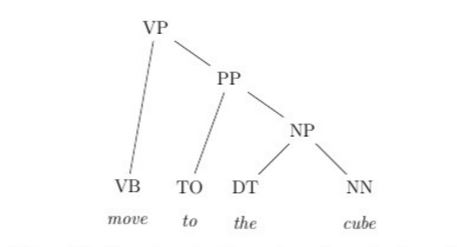
\includegraphics[width=0.45\textwidth]{parse_tree}
\caption{The parse tree for the command ``move to the cube''}
\label{fig:parse_tree}
\end{subfigure}
\vskip2ex
\begin{subfigure}[b]{\columnwidth}
\centering
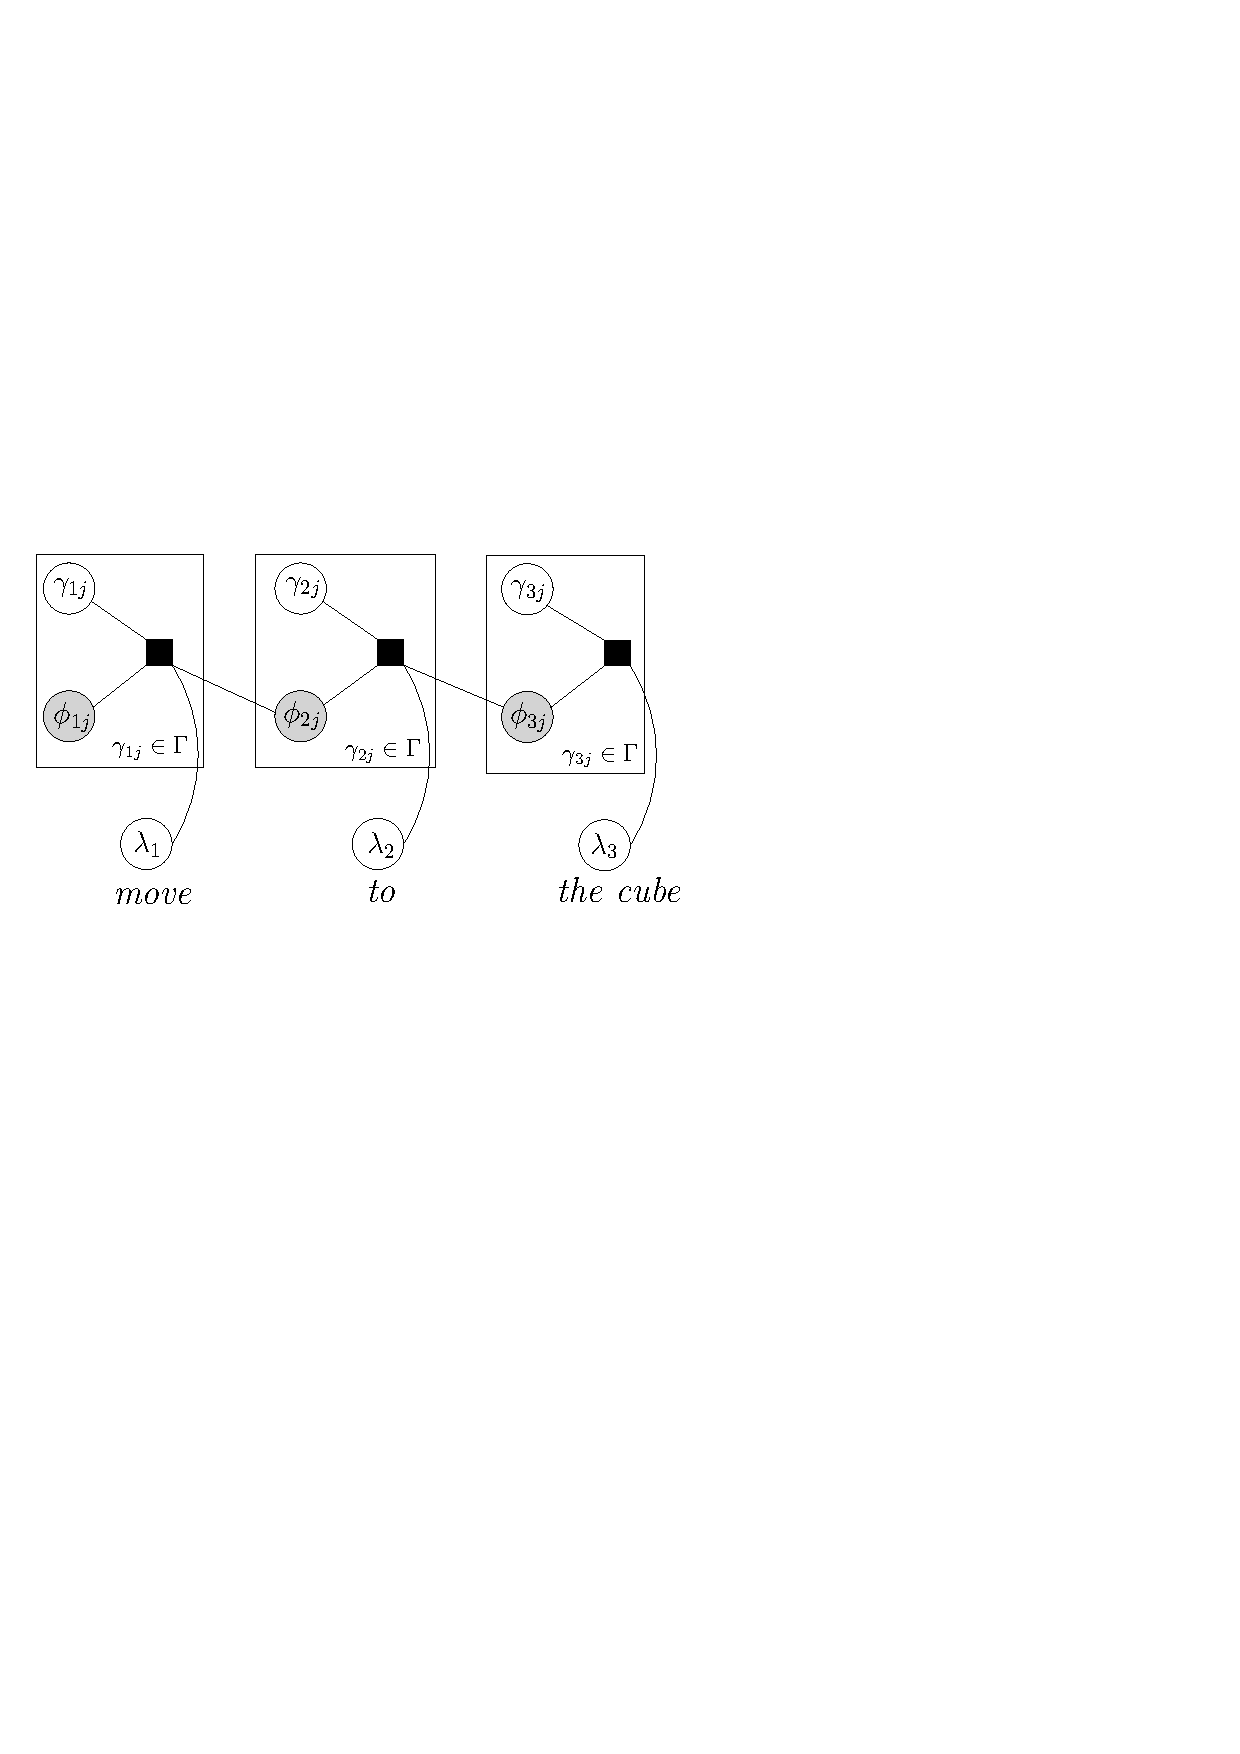
\includegraphics[width=0.7\textwidth]{dcg_plates_new.pdf}
\caption{The DCG graphical model for the parse tree in Fig.~\ref{fig:parse_tree}}
\label{fig:dcg_plates}
\end{subfigure}
\caption{An illustration of a parse tree and the corresponding DCG model where the graph topology of (b) is derived from the structure in (a). In the DCG model, the gray nodes are the observed variables (i.e., the correspondence variables), the white nodes in the plates are the unobserved variables (i.e., the grounding symbols), and the black nodes denote the factors (i.e., representing the conditional relationship between the variables)}
%\vskip-2.5ex
\end{figure}

Finally, the equation in \eqref{eq:dcg_factored1} can be factored as \eqref{eq:llm1}, where the factor function $\Psi : \Phi \times \Gamma \times \Lambda \times \Phi \times \Upsilon \rightarrow
 \mathbb{R}$ (e.g., within each plate in Fig.~\ref{fig:dcg_plates}) determines the most likely configuration $\boldsymbol{\phi^*}=\{\phi_{11}, \phi_{12}, \dots\}$ (where each $\phi_{ij} \in \Phi$) given $\gamma_{ij} \in \Gamma^i$, $\lambda_i \in \boldsymbol\lambda$, $\Phi_{c_{i}} \subset \Phi$, and $\Upsilon_{KP} \subset \Upsilon$. %Accordingly, one may rewrite \eqref{eq:dcg_factored1} as
%In order to expose the use of $\Psi$, one may rewrite Equation~\ref{eq:dcg_factored1} as Equation~\ref{eq:llm1}, \\
\begin{equation}
\boldsymbol{\phi}^* = \argmax_{\phi_{ij} \in \Phi} \prod_{i}^{\boldsymbol{|\lambda|}} \prod_{j}^{|\Gamma^i|} \Psi(\phi_{ij},\gamma_{ij},\lambda_i,\Phi_{c_{i}},\Upsilon_{KP}).
\label{eq:llm1}
\end{equation}

In \eqref{eq:llm1}, the factor function $\Psi$ is a log-linear model composed of a weighted combination of binary functions, that is,
\begin{equation}
\Psi(.) = \frac {\exp \Big( \sum\limits_{f \in F_{DCG}} \mu_f f(\phi_{ij},\gamma_{ij},\lambda_i,\Phi_{c_{i}},\Upsilon_{KP}) \Big)}{\sum\limits_{\phi_{ij} \in \{-1,0,1\}}\exp \Big( \sum\limits_{f \in F_{DCG}} \mu_f f(\phi_{ij},\gamma_{ij},\lambda_i,\Phi_{c_{i}},\Upsilon_{KP}) \Big)},
%\Psi(\phi_{ij},\gamma_{ij},\lambda_i,\Phi_{c_{i}},\Upsilon_{KP}) = \frac {\exp \Big( \sum\limits_{f \epsilon F} \mu_f f(\phi_{ij},\gamma_{ij},\lambda_i,\Phi_{c_{i}},\Upsilon_{KP}) \Big)}{\sum\limits_{\phi_{ij} \in \{-1,0,1\}}\exp \Big( \sum\limits_{f \epsilon F} \mu_f f(\phi_{ij},\gamma_{ij},\lambda_i,\Phi_{c_{i}},\Upsilon_{KP}) \Big)},
\label{eq:llm2}
\end{equation}
where $F_{DCG}$ is the set of hand-coded binary features that evaluate specific traits about a grounding. For example, a linguistic feature can express whether the word ``cube'' appears in the command $\boldsymbol{\lambda}$, or a geometric feature can identify the spatial characteristics of object aggregations (e.g., whether a region corresponds to the area between two objects). Moreover, each $f$ has a corresponding weight $\mu_f$. In the DCG model, the weights $\mu_f$ are learned by maximizing the training set likelihood using a stochastic gradient descent algorithm (i.e., the L-BFGS algorithm\footnote{In our work, we also use the {L-BFGS} algorithm to learn the weights of the feature functions} \cite{liu1989}). 

%  via learning,the weighting of each $f$. In this work,
%the weights $\mu_f$ are learned in a training procedure via .% to generate a more nuanced function that evaluates how likely a phrase is to correspond to a grounding.

Note that a limitation of the DCG model is that it assumes the set of symbols (i.e., objects and phrases) are defined a priori so it does not explicitly represent the unknown symbols. Thus, this model is unable to reason about objects and phrases that have not been trained on. 